\documentclass[12pt, a4paper]{article}

\usepackage[utf8]{inputenc}
\usepackage[T1]{fontenc}
\usepackage[russian]{babel}
\usepackage[oglav,spisok,boldsect, figwhole]{./style/fn2kursstyle1}
\graphicspath{{./style/}{./figures/}}
%\usepackage{float}%"Плавающие" картинки
\usepackage{multirow}
\usepackage{subcaption}
\usepackage{float}%"Плавающие" картинки
%Римские цифры
\newcommand{\RomanNumeralCaps}[1]
{\MakeUppercase{\romannumeral #1}}

\usepackage{enumitem} 
\usepackage{amsmath}
\usepackage{comment}
\usepackage{makecell}

%Параметры титульника
\title{Методы численного решения обыкновенных дифференциальных уравнений}
\group{ФН2-62Б}
\author{З.И.~Абрамов, Г.А. Швецов}
\supervisor{С.А.~Конев}
\date{2023}
\begin{document}
	\newcommand{\pl}{\partial}
	\maketitle
	
	\tableofcontents
	
	\newpage
	
	\section{Контрольные вопросы}
	
	\begin{enumerate}
		\item \textit{Сформулируйте условия существования и единственности решения задачи Коши для обыкновенных дифференциальных уравнений. Выполнены ли они для вашего варианта задания?}
		\smallskip
		
		% О Липшиц-непрерывности в какой норме вы говорите? Объясните геометрический смысл условия Липшица в контексте решения задачи Коши, где u и f — скалярные функции.
		
		% взял из Галанина и немного из лекций по дифурам
		Пусть функция $f(x, u)$ определена и непрерывна в прямоугольнике:
		\[
		D = \{(x, u): |x-x_0| \le a, |u_i - u_0^i| \le b, i = 1, 2, \dots, n\}.
		\]
		
		При этих условиях в прямоугольнике $D$ все компоненты $|f_i| \le M$. Пусть функция $f(x, u)$ является липшиц-непрерывной (по октаэдрической норме) с постоянной $L$ по переменным $u_1$, $u_2$, \dots, $u_n$:
		\[
		|f(x, u^{(1)}) - f(x, u^{(2)})| \le L \sum_{i=1}^n |u_i^{(1)} - u_i^{(2)}| \quad \forall (x, u^{(1)}), (x, u^{(2)}) \in D.
		\]
		
		Тогда существует единственное решение задачи Коши
		\[
		\begin{cases}
			u' = f(x, u), \quad x > x_0, \\
			u(x_0) = u_0,
		\end{cases}
		\]
		где $u$ и $f$ --- вектор-функции из $n$ компонент, на участке
		\[
		|x-x_0| \le \tilde{x}_0 = \min\{a, \frac{b}{M}, \frac1L\}.
		\]
		
		% Для существования решения достаточно непрерывности (из лекции по дифурам).
		% http://w.ict.nsc.ru/books/textbooks/akhmerov/ode_unicode/m-22/m-22.html
		Для функции $f:D \subset \mathbb{R} \to \mathbb{R}$ условие Липшица геометрически можно трактовать как ограниченность по модулю угловых коэффициентов всех хорд графика функции $f$:
		\[
		\left|\frac{f(x) - f(y)}{x-y}\right| \le L.
		\]
		
		\begin{figure}[!h]
			\centering
			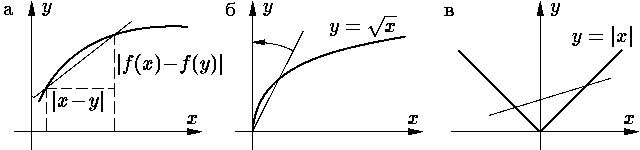
\includegraphics[width=0.7\linewidth]{lipshich}
			%\caption{}
			\label{lipshich}
		\end{figure}
		
		Выражение в левой части неравенства — это угловой коэффициент хорды.
		
		Например, функция $y = \sqrt{x}$ на отрезке $[0, 1]$ не удовлетворяет условию Липшица, т.к. вблизи точки x = 0 хорды графика становятся сколь угодно близкими к вертикали. Функция $y = |x|$ (не всюду дифференцируемая) удовлетворяет условию Липшица с константой $L = 1$, т.к. угловой коэффициент хорд графика, очевидно, по модулю не больше единицы.
		
		Для задачи Коши в случае скалярных функций $u$ и $f$ с двумя начальными условиями
		\[
		\begin{cases}
			u_1' = f(x, u_1), \\
			u_1(x_0) = u_{1,0},
		\end{cases} \qquad \textrm{ и } \qquad \begin{cases}
			u_2' = f(x, u_2), \\
			u_2(x_0) = u_{2,0},
		\end{cases}
		\]
		условие Липшица можно трактовать как
		\[
		|u_1(x) - u_2(x)| \le |u_{1,0} - u_{2,0}| e^{L |x-x_0|},
		\]
		т.е. решения задачи Коши с близкими начальными условиями будут близки при всех $x$, при которых они определены.
		
		Если функция $f$ ограничена, т.е. $|f| \le M$ в области $D$, то
		\begin{comment}
			\begin{multline*}
				|u(x) - u_0| = \left|\int_{x_0}^{x} f(x, u(x)) \textup dx\right| \le \int_{x_0}^{x} |f(x, u(x))| \textup dx \le \\
				\le \int_{x_0}^{x} M \textup dx = M (x-x_0) \le M a,
			\end{multline*}
		\end{comment}
		\[
		|u(x) - u_0| = \left|\int_{x_0}^{x} f(x, u(x)) \textup dx\right| \le \int_{x_0}^{x} |f(x, u(x))| \textup dx \le \int_{x_0}^{x} M \textup dx = M |x-x_0|,
		\]
		%где $x_0 \in [x_0; x_0 + a]$, $[x_0; x_0 + a]$ --- отрезок интегрирования. Таким образом, из ограниченности правой части следует то, что решение $u(t)$ отличается от начального условия $u_0$ не более чем на $M a$, т.е. множество решения $(x, u(x))$ лежит в прямоугольнике $G = \{x_0 \le x \le x_0 + a; u_0 - M a \le u(x) \brop\le u_0 + M a\}$.
		% https://ahiin.livejournal.com/12469.html
		где $|x-x_0| \le a$ --- отрезок интегрирования. Таким образом, из ограниченности правой части следует то, что решение $u(t)$ лежит внутри плоского конуса с вершиной в точке $(x_0, u_0)$ и образующими, имеющие угловые коэффициенты $M$ и $-M$.
		
		Отметим, что если $f$ непрерывно дифференцируема в $D$ по $u_1$, \dots, $u_n$, то она является липшиц-непрерывной по этим переменным.
		
		Правая часть системы Ван-дер-Поля бесконечно дифференцируема по $y_1$ и $y_2$ во всем пространстве $\mathbb{R}^2$, т.е. для нее выполняется указанная теорема.
		
		Классы функций:
		\begin{enumerate}
			\item Аналитические функции
			\item Бесконечно дифференцируемые функции
			\item Липшиц-непрерывные функции
			\item Дифференцируемые функции
			\item Непрерывно дифференцируемые функции
			\item Непрерывные функции
		\end{enumerate}
		
		Покажем вложенность классов друг в друга:	
		\[\textup a\subset\textup b\subset\textup e\subset\begin{matrix}\textup d \\ \textup c\end{matrix}\subset\textup f.\]
		
		\item \textit{Что такое фазовое пространство? Что называют фазовой траекторией? Что называют интегральной кривой?}
		\smallskip
		
		Рассмотрим систему обыкновенных дифференциальных уравнений $n$-го порядка $u' = f(x, u)$, и пусть вектор-функция $u = F(x)$ --- решение системы, определенное на промежутке $[a, b]$.
		
		Множество точке $F(x)$, $x \in [a, b]$ есть кривая в пространстве $\mathbb{R}_{u^n}$. Эту кривую называют \textbf{фазовой траекторией системы} (или просто траекторией, или фазовой кривой), а пространство $\mathbb{R}_{u^n}$, в котором расположены фазовые траектории, называют \textbf{фазовым пространством системы}.
		
		\looser{-0.02}{\textbf{Интегральная кривая системы} определяется уравнением} $u = F(x)$, $x \in [a, b]$ и изображается в $(n+1)$-мерном пространстве $\mathbb{R}_{x, u^n}$.
		
		\looser{-0.02}{Фазовая траектория --- это проекция интегральной кривой на пространство $\mathbb{R}_{u^n}$.}
		
		\item \textit{Каким порядком аппроксимации и точности обладают	методы, рассмотренные в лабораторной работе?}
		\smallskip
		
		В данной лабораторной работе представлены три метода четвертого порядка точности: \textit{Метод Рунге -- Кутты, Адамса -- Башфорта, <<прогноз-коррекция>>}. Также рассматриваюся \textit{явный и неявный методы Эйлера} первого порядка точности, а также \textit{симметричная схема} и \textit{метод Рунге -- Кутты} второго порядка. Во всех случаях порядок точности совпадает с порядком аппроксимации.
		
		% Обратите внимание: при вычислении погрешностей аппроксимации методов вы утверждаете, что используете разложение в ряд Тейлора. Каковы условия сходимости ряда Тейлора?
		\textbf{Условие сходимости ряда Тейлора.} Для того чтобы бесконечно дифференцируемая в точке $a$ функция $f(x)$ являлась суммой составленного для нее ряда Тейлора, необходимо и достаточно, чтобы \[\lim\limits_{n\to\infty}R_n(x)=0,\;R_n(x)=\frac{f^{(n+1)}(\xi)}{(n+1)!}(x-a)^{n+1},\;\xi \in (a,x).\]
		
		%\textbf{Теорема.} Если функция $f(x)$ имеет непрерывные производные вплоть до $n+1$ порядка в окрестности точки $x_0$, то она представима в виде ряда Тейлора в окрестности этой точки:
		%\[ f(x) = f(x_0) + f'(x_0) (x-x_0) + \dots + \frac1{n!} f^{(n)}(x_0) (x-x_0)^n + o(|x-x_0|^n),\]
		%где $o(|x-x_0|^n)$ --- остаточный член в форме Пеано.
		
		Покажем, что явный метод Эйлера обладает первым порядком аппроксимации:
		\begin{multline*}
			\psi_h^{(1)} = f(t_n, u_n) - \frac{u_{n+1}-u_n}{\tau} = |\text{раскл. $u_{n+1}$ в ф-ле Тейлора}, f(t_n, u_n) = u_n'| = \\
			= u_n' - \frac1\tau \left(u_n + \tau u_n' + O(\tau^2) - u_n \right) = u_n' - u_n' - \frac1\tau O(\tau^2) = O(\tau).
		\end{multline*}
		
		Аналогично для неявного метода Эйлера. Разница лишь в том, что вместо $u_{n+1}$ мы раскладываем в ряд $u_n$.
		\begin{multline*}
			\psi_h^{(1)} = f(t_{n+1}, u_{n+1}) - \frac{u_{n+1}-u_n}{\tau}  = u_{n+1}' - \frac1\tau \left(u_{n+1} - u_{n+1}  - (-\tau) u_{n+1}' - O(\tau^2) \right) = \\
			= u_{n+1}' - u_{n+1}' + \frac1\tau O(\tau^2) = O(\tau).
		\end{multline*}
		
		Пользуясь тем же аппаратом, приходим к тому, что симметричная схема имеет второй порядок аппроксимации. В этом случае разложение происходит в серединной точке $t_n + \tau/2$. Значения точного решения $u(t)$ и его производных в этой точке будут иметь индекс $n+1/2$.
		\begin{multline*}
			\psi_h^{(1)} = \frac{f(t_n, u_n) + f(t_{n+1}, u_{n+1})}2 - \frac{u_{n+1} - u_n}\tau = \frac{u_n' + u_{n+1}'}2 - \frac{u_{n+1} - u_n}\tau = \\
			= \frac12\left(u_{n+\frac12}' - \frac\tau2 u_{n+\frac12}'' + O(\tau^2) + u_{n+\frac12}' + \frac\tau2 u_{n+\frac12}'' + O(\tau^2)\right) - \\
			- \frac1\tau \left( u_{n+\frac12} + \frac\tau2 u_{n+\frac12}' + \frac{\tau^2}8 u_{n+\frac12}'' + O(\tau^3)  - u_{n+\frac12} + \frac\tau2 u_{n+\frac12}' - \frac{\tau^2}8 u_{n+\frac12}'' - O(\tau^3)\right) = \\
			= \frac12\left(u_{n+\frac12}' + u_{n+\frac12}'\right)  + O(\tau^2) - \frac1\tau \tau u_{n+\frac12}' + O(\tau^2) = u_{n+\frac12}' - u_{n+\frac12}' + O(\tau^2) = O(\tau^2).
		\end{multline*}
		
		% Покажите, что метод прогноза и коррекции, рассматриваемый в лабораторной работе, обладает четвёртым порядком сходимости
		
		%Предиктор в методе <<прогноз-коррекция>> в виде явного метода Адамса находит приближение с 4 порядком сходимости. Т.к. корректор также обладает 4 порядком, то при выполнении условий сходимости метода простой итерации можно утверждать, что новое приближение будет иметь порядок точности не хуже и что комбинация этих методов будет давать 4 порядок.
		Показать четвертый порядок аппроксимации метода <<прогноз-коррекция>> можно тем, что в 6 контрольном вопросе для данного метода было получено, что погрешность аппроксимации имеет слагаемые порядка не ниже 4.
		
		\item \textit{Какие задачи называются жесткими? Какие методы предпочтительны для их решения? Какие из рассмотренных методов можно использовать для решения жестких задач?}
		\smallskip
		
		Систему ОДУ $u' = A u$ с постоянной матрицей $A = A_{m\times m}$ называют жесткой, если
		\begin{itemize}
			\item все собственные значения матрицы $A$ имеют отрицательную действительную часть, т.е. $\mathrm{Re}\,\lambda_i < 0$, $\lambda_i \in \sigma(A)$, $i = \overline{1, m}$.
			\item число $S$, называемое числом жесткости, велико:
			\[
			S = \frac{\max\limits_{1 \le k \le m} |\mathrm{Re}\,\lambda_k|}{\min\limits_{1 \le k \le m} |\mathrm{Re}\,\lambda_k|}.
			\]
		\end{itemize}
		
		Если матрица $A$ не постоянна и $\lambda_k = \lambda_k(t)$, то вводят понятие числа жесткости системы ОДУ на временном интервале. В этом случае должно быть велико значение $\sup\limits_{t\in(0,T)} S(t)$.
		
		% Что означает фраза «число S велико»? Зачем для решения жёстких задач применяют A-устойчивые методы? Дайте определение A-устойчивого метода. В чём смысл определения A-устойчивости?
		
		Понятие <<$S$ велико>> относительно и зависит в первую очередь от применяемого численного метода и того, с насколько большим шагом предпочтительно решать задачу.
		
		Областью устойчивости метода решения задачи Коши называется множество точек $\mu = \lambda \tau$ комплексной плоскости, для которых данный метод применительно к уравнению $u' = \lambda u$ устойчив. Иными словами, должно быть справедливо неравенство $|y_{n+1}| \le |y_n|$, что выполняется, если корни характеристического уравнения лежат внутри единичного круга $|q| \le 1$, а на его границе нет кратных корней.
		
		Для решения жестких систем предпочтительно использовать $A$-устойчивые методы, т.е. методы, у которых область устойчивости содержит левую полуплоскость $\mathrm{Re}\,\mu < 0$. Это связано с тем, что при решении систем вида $u' = A u$, где $A$ --- диагональная матрица (при произвольной матрице можно сделать замену переменных, при которых матрица правой части будет диагональной), может возникнуть ситуация, когда для разных уравнений $u_i' = \lambda_i u_i$ для достижения определенной точности лучше использовать сильно разные шаги $\tau$, что невозможно, поскольку для всей системы нужно использовать одинаковый шаг. Более того при использовании некоторых методов, например, на уравнениях $u' = \lambda u$, где $\mathrm{Re}\,\mu < 0$, могут возникать ситуации, когда численное решение ведет себя некорректно, сильно отклоняясь от аналитического на каждом шаге. $A$-устойчивые методы в этих случаях (при $\mathrm{Re}\,\mu < 0$) дают разумное сеточное решение, стремящееся к нулю.
		% Лукин, стр. 328
		%В качестве примера можно привести следующую задачу Коши:
		\begin{comment}
			\begin{equation*}
				\begin{cases}
					u_1'(t) = -u_1(t), \\
					u_2'(t) = -\varepsilon u_2(t), t > 0,\\
					u_1(0) = u_{1,0}, u_2(0) = u_{2,0}.
				\end{cases}
			\end{equation*}
		\end{comment}
		
		
		Среди рассмотренных методов к $A$-устойчивым относятся неявный метод Эйлера и симметричная схема.
		
		% Покажите, что явный метод Эйлера и явные методы Рунге — Кутты из этой лабораторной работы не являются A-устойчивыми.
		
		Найдем область устойчивости явного метода Эйлера.
		\begin{eqnarray*}
			& \dfrac{y_{n+1} - y_n}\tau = f(t_n, y_n), \quad f(t, y) = \lambda y \\
			& q-1 = \tau \lambda, \quad q = 1 + \mu, \quad \mu = \mu_x + i \mu_y, \\
			& |q|^2 = (1+\mu_x)^2 + \mu_y^2 \le 1.
		\end{eqnarray*}
		
		Область устойчивости представляет собой круг единичного радиуса с центром в точке $(-1; 0)$, т.е. метод не является $A$-устойчивым.
		
		Теперь построим область устойчивости двухстадийного метода Рунге --- Кутты второго порядка:
		\[
		k_1 = f(t_n, y_n), \quad k_2 = f(t_n + \tau, y_n + \tau k_1), \quad y_{n+1} = y_n + \frac\tau2 k_1 + \frac\tau2 k_2.
		\]
		
		Запишем метод применительно к уравнению Далквиста $u' = \lambda u$:
		\[
		k_1 = \lambda y_n, \quad k_2 = \lambda \left(y_n + \tau \lambda y_n \right), \quad y_{n+1} = y_n \left(1 + \frac\tau2 \lambda + \frac\tau2 (\lambda + \tau \lambda^2) \right).
		\]
		
		Для устойчивости метода необходимо, чтобы $|R(\mu)| \le 1$, где $R(\mu)$ --- функция устойчивости:
		\[
		R(\mu) = 1 + \mu + \frac{\mu^2}2, \quad \mu \in \mathbb{C}.
		\]
		
		Множество $|R(\mu)| \le 1$ изображено на рис.~\ref{rk2}. Из него видно, что метод не является $A$-устойчивым.
		
		\begin{figure}[H]
			\centering
			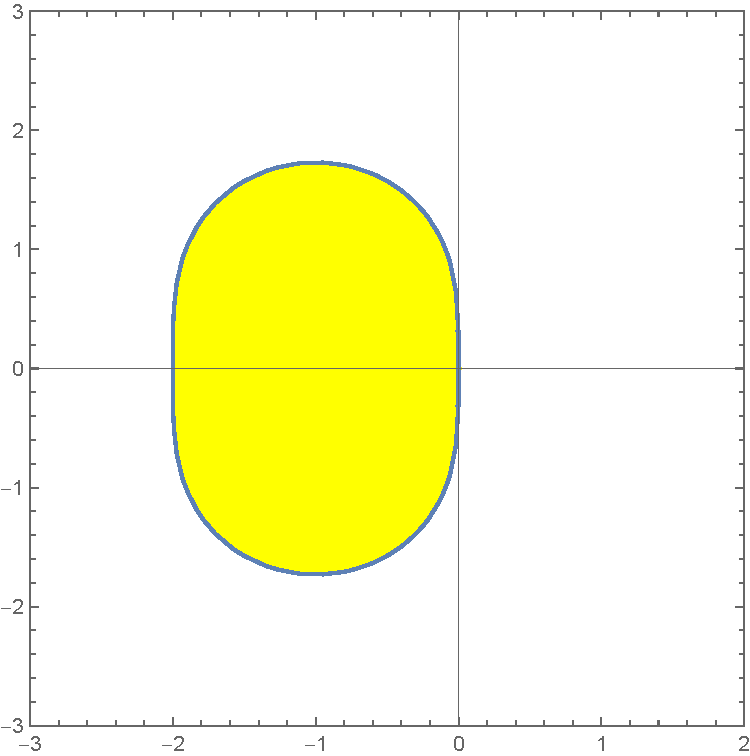
\includegraphics[width=0.6\textwidth]{rk2}
			\caption{Область устойчивости метода Рунге --- Кутты второго порядка}
			\label{rk2}
		\end{figure}
		
		Для аналогичного метода с формулами
		\[
		k_1 = f(t_n, y_n), \quad k_2 = f(t_n + \frac\tau2, y_n + \frac\tau2 k_1), \quad y_{n+1} = y_n \tau k_2
		\]
		получается такая же функция устойчивости \cite{lukin}, т.е. и область устойчивости одна и та же. Также из этого следует, что метод не является $A$-устойчивым.
		
		Для метода Рунге --- Кутты четвертого порядка с расчетными формулами
		\begin{eqnarray*}
			& k_1 = f(t_n, y_n), \quad k_2 = f(t_n + \frac\tau2, y_n + \frac\tau2 k_1), \quad k_3 = f(t_n + \frac\tau2, y_n + \frac\tau2 k_2),\\
			& k_4 = f(t_n + \tau, y_n + \tau k+3), \quad  y_{n+1} = y_n + \frac\tau6 \left(k_1 + 2 k_2 + 2 k_3 + k_4\right)
		\end{eqnarray*}
		имеет функцию устойчивости (вычислена в Wolfram Mathematica)
		\[
		R(\mu) = 1 + \mu + \frac{\mu^2}2 + \frac{\mu^3}6 + \frac{\mu^4}{24}.
		\]
		
		Область устойчивости изображена на рис.~\ref{rk4}. Метод не является $A$-устойчивым.
		
		\begin{figure}[H]
			\centering
			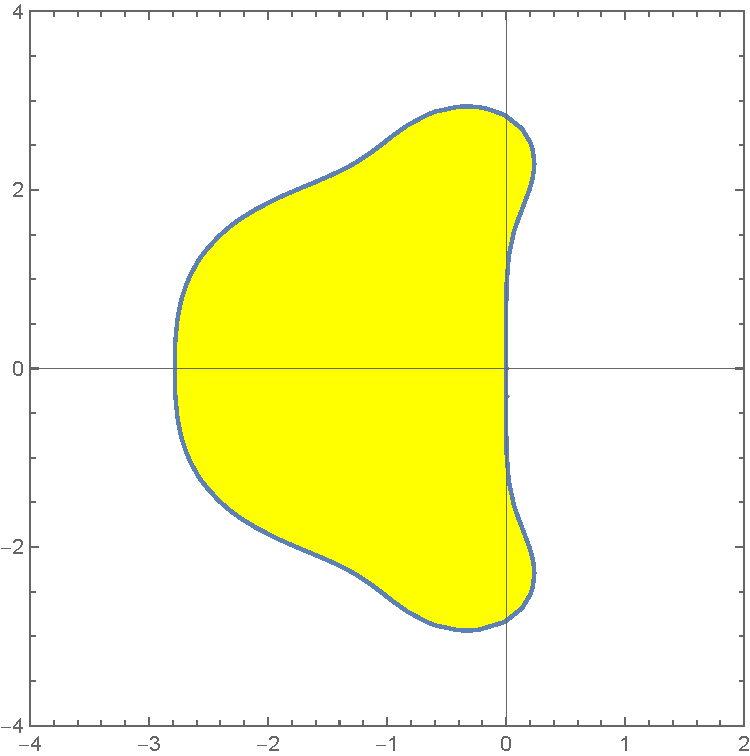
\includegraphics[width=0.6\textwidth]{rk4}
			\caption{Область устойчивости метода Рунге --- Кутты второго порядка}
			\label{rk4}
		\end{figure}
		
		% Можете ли вы доказать, что среди линейных явных многошаговых методов нет ни A-устойчивых, ни A(alpha)-устойчивых?
		
		Для явных методов коэффициент $b_0 = 0$. Из характеристического уравнения получаем, что для любого $q$ справедливо равенство
		\[
		\mu = \sum_{k=0}^m a_k q^{m-k} \Big/ \sum_{k=1}^m b_k q^{m-k}.
		\]
		
		Из этого следует, что при больших по модулю значениях $q$ параметр $\mu$ возрастает линейно как $(a_0/b_1)q$, если $b_1 \neq 0$, либо как более высокая степень $q$, если $b_1 = 0$. Следовательно, для любого достаточно большого $\mu$ найдется $q$ из левой полуплоскости, в том числе с $|q| > 1$, для которого справедливо характеристическое уравнение. В результате $A$-устойчивость отсутствует. Такие же соображения доказывают, что ни для какого $\alpha$ не существует явного $A(\alpha)$-устойчивого линейного многошагового метода.
		
		\item \textit{Как найти $\vec y_1,\,\vec y_2,\,\vec y_3$, чтобы реализовать алгоритм прогноза и коррекции?}
		\smallskip
		
		Для нахождения значений $\vec y_1,\,\vec y_2,\,\vec y_3$ требуется использовать одношаговый метод. Причем точность метода должна совпадать с точностью многошагового метода, который мы хотим реализовать. В данной лабораторной работе для реализации методов четвертого порядка Адамса --- Башфорта и <<прогноза и коррекции>> мы использовали метод Рунге --- Кутты четвертого порядка.
		
		% С каким порядком должен быть найден y1, если мы решаем задачу с помощью симметричной схемы? А y1, y2, y3 — в случае явного четырёхшагового метода Адамса из работы?
		
		Приведем без доказательства следующую теорему.
		
		\textbf{Теорема.} Пусть разностный $m$-шаговый метод удовлетворяет условию корней (т.е. является нуль-устойчивым) и $|f_y'| \le L$. Тогда для любого $m\tau \le t_n = n\tau \le T$ при достаточно малом $\tau$ выполнена оценка
		\[
		|y_n - u(t_n)| \le M \left(\max_{0\le j \le m-1} |y_j - u(t_j)| + \max_{m \le j \le n} \left|\psi_{h,j}^{(1)}\right|\right),
		\]
		где $M$ --- постоянная, не зависящая от $m$; $|y_j - u(t_j)|$, $j = \overline{0, m-1}$, --- погрешность в задании начальных условий; $\psi_{h,j}^{(1)}$, $j = \overline{m, n}$, --- невязка (погрешность аппроксимации).
		
		Из этой теоремы следует, что порядок сходимости напрямую зависит от порядка метода, находящего $y_j$, $j = \overline{0, m-1}$. При этом все методы Адамса являются нуль-устойчивыми. Из-за этого значения $y_1$, $y_2$, $y_3$ для явного четырехшагового метода Адамса требуется искать методом хотя бы четвертого порядка, чтобы сохранить этот же порядок для самого метода Адамса.
		
		Симметричная схема является неявным методом Адамса второго порядка. Поэтому вследствие этой же теоремы, чтобы сохранить второй порядок сходимости, $y_1$ должно быть найдено хотя бы со вторым порядком, что накладывает ограничения на метод, находящий корень нелинейного алгебраического уравнения. Для симметричной схемы подходит, например, метод Ньютона, имеющий как раз второй порядок.
		
		% На основании чего вы утверждаете, что начальные приближения yi, i = 1, 2, 3 надо искать с четвёртым порядком точности?
		
		Для достижения 4 порядка точности методом прогноза и коррекции требуется, чтобы предиктор имел порядок не меньше. Это необходимо, т.к. корректор не работает до срабатывания условия точности, а выполняет только один шаг, т.е. сам по себе он  не способен обеспечить нужный порядок. При этом нужно учесть, что предиктором является явный метод Адамса, для которого $y_1$, $y_2$, $y_3$ необходимо искать методом 4 порядка, как уже было написано ранее. Таким образом, в методе <<прогноз-коррекция>> $y_1$, $y_2$, $y_3$ также, как и в случае явного метода Адамса, нужно искать с 4 порядком точности.
		
		\item \textit{Какой из рассмотренных алгоритмов является менее трудоемким? Какой из рассмотренных алгоритмов позволяет достигнуть заданную точность, используя наибольший	шаг интегрирования? Какие достоинства и недостатки рассмотренных алгоритмов вы можете указать?}
		\smallskip
		
		\textbf{Явный метод Эйлера}
		
		\textit{Достоинства:}
		
		\begin{itemize}
			\item является самым простым методом решения обыкновенных дифференциальных уравнений, реализуется элементарным образом;
			\item на одной итерации требуется вызывать всего лишь один раз функцию $f$.
		\end{itemize}
		
		\textit{Недостатки:}
		
		\begin{itemize}
			\item низкий порядок точности (первый);
			\item не подходит для решения жестких задач.
		\end{itemize}
		
		\textbf{Неявный метод Эйлера}
		
		\textit{Достоинства:}
		
		\begin{itemize}
			\item подходит для решения жестких задач, т.к. обладает $A$-устойчивостью. 
		\end{itemize}
		
		\textit{Недостатки:}
		
		\begin{itemize}
			\item обладает лишь первым порядком точности;
			\item на каждом шаге требуется решать в общем случае систему нелинейных уравнений, что сильно повышает количество вызовов функции правой части ДУ.
		\end{itemize}
		
		\textbf{Симметричная схема}
		
		\textit{Достоинства:}
		
		\begin{itemize}
			\item является $A$-устойчивым методом;
			\item легко реализуется путем модификации неявного метода Эйлера, вследствие чего повышается порядок точности с первого до второго.
		\end{itemize}
		
		\textit{Недостатки:}
		
		\begin{itemize}
			\item требует на каждом шаге решать систему нелинейных уравнений;
			\item второго порядка точности часто бывает недостаточно.
		\end{itemize}
		
		\textbf{Классический метод Рунге --- Кутты 4 порядка}
		
		\textit{Достоинства:}
		
		\begin{itemize}
			\item обладает четвертым порядком сходимости, что является самым большим среди рассмотренных методов;
			\item имеет самую большую область устойчивости среди рассмотренных явных методов.
		\end{itemize}
		
		\textit{Недостатки:}
		
		\begin{itemize}
			\item слабо подходит для решения жестких задач;
			\item требует на каждом шаге вычисления четырех раз функции правой части (больше остальных рассмотренных явных методов).
		\end{itemize}
		
		\textbf{Метод Адамса --- Башфорта 4 порядка}
		
		\textit{Достоинства:}
		
		\begin{itemize}
			\item имеет четвертый поряд точности;
			\item на одном шаге требуется вычислять всего один раз функцию $f$.
		\end{itemize}
		
		\textit{Недостатки:}
		
		\begin{itemize}
			\item является условно устойчивым (причем область устойчивости меньше только у явного метода Эйлера), вследствие чего плохо подходит для решения жестких задач;
			\item требует реализации дополнительного метода решения ОДУ для вычисления приближенного решения на первых трех шагах.
		\end{itemize}
		
		\textbf{Метод <<прогноз-коррекция>> 4 порядка}
		
		\textit{Достоинства:}
		
		\begin{itemize}
			\item имеет четвертый поряд точности;
			\item при нахождении следующего приближения нужно вычислять функцию $f$ два раза, что меньше, чем у метода Рунге --- Кутты.
			\item имеет значительно большую область устойчивости, чем у метода Адамса --- Башфорта.
		\end{itemize}
		
		\textit{Недостатки:}
		
		\begin{itemize}
			\item является условно устойчивым;
			\item так как данный метод основан на методе простой итерации, то он требует от функции $f$ дополнительные условия для сходимости;
			\item требует реализации дополнительного метода решения ОДУ для вычисления приближенного решения на первых трех шагах.
		\end{itemize}
		\begin{table}[H]
			\caption{Трудоемкость методов за один шаг}
			\footnotesize
			\begin{center}
				\begin{tabular}{|c|c|c|c|}
					\hline
					\makecell{Метод}&\makecell{Вычисления функций\\ правой части}&\makecell{Умножение вектора\\ на число}&\makecell{Векторные операции\\ сложения}\\
					\hline
					Эйлера (явный)&$1$&$1$&$1$\\
					\hline
					Эйлера (неявный)*&---&---&---\\
					\hline
					Симметрическая схема*&---&---&---\\
					\hline
					Рунге --- Кутта (2)&$2$&$2$&$2$\\
					\hline
					Рунге --- Кутта (4)&$4$&$6$&$10$\\
					\hline
					Адамса --- Башфорта**&1&5&4\\
					\hline
					<<Прогноз-коррекция>>**&2&9&8\\
					\hline
				\end{tabular}
			\end{center}
		\end{table}
		* Из-за применения внутреннего алгоритма, решающего нелинейное уравнение, нельзя сказать, какое именно количество операций будет выполнено на одном шаге.
		
		** Метод используется после подготовки одношаговыми методами.
		
		Таким образом, исходя из таблицы, менее трудоемким методом на один шаг является явный метод Эйлера.
		
		% Какой из рассмотренных алгоритмов позволяет достигнуть заданную точность, используя наибольший шаг интегрирования?
		
		Найдем в погрешности аппроксимации слагаемые более высокого порядка путем замены в вычислительной схеме $\tau$ на $\alpha \tau$. Далее разложим сеточную функцию $\psi_h^{(1)}$ по $\alpha$ в нуле до более высокой степени, чем при обычном вычислении порядка аппроксимации, и примем $\alpha = 1$. Покажем приведенный процесс на примере явного метода Эйлера:
		\begin{multline*}
			\psi_h^{(1)} = \left[f(t_n, u_n) - \frac{u_{n+1}-u_n}{\alpha\tau}\right]\Bigg|_{\alpha = 1} = \\
			= \left[u_n' - \frac1\tau \left(u_n + \alpha\tau u_n' + \frac12(\alpha\tau)^2 u_n'' + O((\alpha\tau)^3) - u_n \right)\right]\Bigg|_{\alpha = 1} =\\
			= u_n' - \frac1\tau \left(u_n + \tau u_n' + \frac12\tau^2 u_n'' - u_n \right) + O(\tau^2) = -\frac12 u_n''\tau + O(\tau^2).
		\end{multline*}
		
		Для остальных методов приведем результаты без вывода (операции были проведены в системе Wolfram Mathematica):
		
		Неявный метод Эйлера: $\psi_h^{(1)} = \sfrac12 u_n''\tau + O(\tau^2)$.
		
		Симметричная схема: $\psi_h^{(1)} = \sfrac1{12} u_n'''\tau^2 + O(\tau^3)$.
		
		Явный метод Адамса: $\psi_h^{(1)} = -\sfrac{251}{720} u_n^{(5)}\tau^4 + O(\tau^5)$.
		
		Метод прогноза и коррекции: $\psi_h^{(1)} = \sfrac{19}{720} u_n^{(5)}\tau^4 + O(\tau^5)$.
		
		Метод Рунге --- Кутты 2 порядка: $\psi_h^{(1)} = -\sfrac1{24} (u_n''' + 3 u_n'' f_u(t_n, u_n))\tau^2 + O(\tau^3)$.
		
		Метод Рунге --- Кутты 4 порядка (для краткости приведем в случае ДУ вида $u' = f(u)$): $\psi_h^{(1)} = \sfrac1{2880}(u_n^{(5)} - 5 u_n^{(4)} f'(u_n) - 5(4 u_n' f'(u_n)^4 - 9 u_n'^2 f'(u_n)^2 f''(u_n) + 2 u_n'^3 f''(u_n)^2)) \tau ^4 + O(\tau^5)$.
		
		Таким образом, среди методов второго порядка нельзя выделить <<победителя>>, т.е. разница между константами незначительная (два раза), но в случае метода Рунге --- Кутты 2 порядка присутствуют дополнительные слагаемые, которые могут вносить существенный вклад. Также можно предположить, что метод <<прогноз-коррекция>> в большинстве случаев будет точнее метода Адамса --- Башфорта. Дополнительно можно выдвинуть предположение, что метод Рунге --- Кутты 4 порядка будет точнее метода прогноза и коррекции, из-за значительно более меньшей константы. Т.е. метод Рунге --- Кутты 4 порядка позволяет достигнуть заданную точность, используя больший шаг интегрирования.
		
		\item \textit{Какие алгоритмы, помимо правила Рунге, можно использовать для автоматического выбора шага?}
		\smallskip
		
		% Галанин, Лукин, стр. 312
		Для выбора шага можно использовать так называемые вложенные методы Рунге --- Кутты. Идея состоит в том, чтобы вместе с приближенным значением решения $y_{n+1}$ вычислять более точное (более высокого порядка) приближение $\hat{y}_{n+1}$, использовав при этом мининимальные вычислительные ресурсы. Для этого можно использовать пару методов Рунге --- Кутты, внутренние стадии которых совпадают (хотя бы частично), т.е. использовать пару методов со следующей таблицей Бутчера:
		\begin{table}[h!]
			\centering
			\begin{tabular}{c|ccccc}
				0 &&&&& \\
				$a_2$ & $b_{21}$ &&&& \\
				$a_3$ & $b_{31}$ & $b_{32}$ &&& \\
				\dots & \dots & \dots & \dots && \\
				$a_m$ & $b_{m1}$ & $b_{m2}$ & \dots & $b_{m,m-1}$ &\\
				\hline
				& $\sigma_1$ & $\sigma_2$ & \dots & $\sigma_{m-1}$ & $\sigma_m$ \\
				& $\hat{\sigma}_1$ & $\hat{\sigma}_2$ & \dots & $\hat{\sigma}_{m-1}$ & $\hat{\sigma}_m$ \\
			\end{tabular}
			%\caption{Caption}
			%\label{tab:my_label}
		\end{table}
		
		% https://www.youtube.com/watch?v=2hrqY5ugBWI&list=PLwL0ZEQK13GOONTaZfaxAFmhLC8Ee2RQ-&index=5
		Тогда если первый метод имеет порядок $p$, а второй --- $\hat{p}$, при этом $\hat{p} > p$, а также предположить, что в качестве $y_n$ взято точное решение, то
		\begin{eqnarray*}
			& u_{n+1} = y_n + h \sum\limits_{i=1}^m \sigma_i k_i + \varepsilon = y_{n+1} + \varepsilon, \quad \varepsilon = O(h^{p+1}), \\
			& u_{n+1} = y_n + h \sum\limits_{i=1}^m \hat{\sigma}_i k_i + \hat{\varepsilon} = \hat{y}_{n+1} + \hat{\varepsilon}, \quad \hat{\varepsilon} = O(h^{\hat{p}+1}).
		\end{eqnarray*}
		
		Вычитая первую строку из второй и перенося $\varepsilon$ и $\hat{\varepsilon}$ вправо, получаем:
		\[
		h \sum\limits_{i=1}^m (\hat{\sigma}_i - \sigma_i) k_i = \varepsilon - \hat{\varepsilon} = \varepsilon + O(h^{\hat{p}+1}).
		\]
		
		Пренебрегая слагаемыми более высокого порядка, получаем формулу для оценки погрешности:
		\[
		\varepsilon \approx \hat{y}_{n+1} - y_{n+1}.
		\]
		
		Отметим, что использование для дальнейших расчетов в качестве значения приближенного решения величины $\hat{y}_{n+1}$ нежелательно, несмотря на ее потенциально более высокую точность. Дело в том, что в таком случае $\varepsilon$ уже не является оценкой погрешности приближенного решения, в связи с чем эта оценка может быть существенна занижена.
		
		% Хайер, Ваннер, стр. 175 - метод Дормана-Принса
		
		% можно написать про метод оценки погрешности через константы M и L
	\end{enumerate}
	\newpage
	\section{Результаты}
	
	В качестве тестового примера возьмем следующую задачу Коши:
	\begin{equation*}
		\begin{cases}
			u'(x) = \frac15 u(x) \ctg\left(\dfrac{x}5\right) + 2 \dfrac{u(x)}{x} + x \sin\left(\dfrac{x}5\right), \\
			u(1) = 0, \quad x \in [1,\, 5].
		\end{cases}
	\end{equation*}
	
	Она имеет аналитическое решение вида
	\begin{equation*}
		u(x) = x^2 \ln(x) \sin\left(\frac{x}5\right).
	\end{equation*}
	
	\subsection{Оценка порядка сходимости}
	
	Сокращенный набор таблиц (только с помощью точного решения и только в узле $t_* = 10\tau$):
	
	\begin{table}[H]
		\caption{Явный и неявный методы Эйлера}
		\centering
		\begin{tabular}{|c|c|c|c||c|c|c|}\hline
			& \multicolumn{3}{c||}{\makecell{Явный м. Эйлера}} & \multicolumn{3}{c|}{Неявный м. Эйлера} \\\cline{2-7}
			$\tau$ & AbsErr($\tau$) & $\Delta$ & $\log_2 \Delta$ & AbsErr($\tau$) & $\Delta$ & $\log_2 \Delta$ \\ \hline
			%0.1 & & & & & \\ \hline
			0.1000000 & 0.218727   &   ---   & ---     & 0.325049&     --- &   ---   \\ \hline
			0.0500000 & 0.119105   & 1.83643 & 0.87690 & 0.144913& 2.24306 & 1.16547 \\ \hline
			0.0250000 & 0.0623276  & 1.91095 & 0.93429 &0.0687332& 2.10834 & 1.07611 \\ \hline
			0.0125000 & 0.0319072  & 1.9534  & 0.96599 &0.0335057& 2.05139 & 1.0366  \\ \hline
			0.0062500 & 0.0161462  & 1.97615 & 0.98269 &0.0165456& 2.02505 & 1.01796 \\ \hline
			0.0031250 & 0.00812212 & 1.98793 & 0.99127 &0.0082220& 2.01237 & 1.0089  \\ \hline
			0.0015625 & 0.00407343 & 1.99393 & 0.99561 &0.0040984& 2.00615 & 1.00443 \\ \hline
		\end{tabular}
	\end{table}
	
	\begin{table}[H]
		\caption{Методы Рунге --- Кутты 2 и 4 порядка}
		\centering
		\begin{tabular}{|c|c|c|c||c|c|c|}\hline
			& \multicolumn{3}{c||}{\makecell{м. РК2}} & \multicolumn{3}{c|}{м. РК4} \\\cline{2-7}
			$\tau$ & AbsErr($\tau$) & $\Delta$ & $\log_2 \Delta$ & AbsErr($\tau$) & $\Delta$ & $\log_2 \Delta$ \\ \hline
			%0.1 & & & & & \\ \hline
			0.1000000 & 0.0145975  &   ---   & ---     & 5.2622e-05&     --- &   ---   \\ \hline
			0.0500000 & 0.003943   & 3.70213 & 1.88835 & 3.68212e-06 & 14.2912 & 3.83706 \\ \hline
			0.0250000 & 0.00102438 & 3.84915 & 1.94454 & 2.43446e-07 & 15.125  & 3.91886 \\ \hline
			0.0125000 &0.000261037 & 3.92427 & 1.97242 & 1.5648e-08  & 15.5576 & 3.95955  \\ \hline
			0.0062500 &6.58838e-05 & 3.96209 & 1.98626 & 9.91786e-10 & 15.7776 & 3.97981 \\ \hline
			0.0031250 &1.65494e-05 & 3.98103 & 1.99314 & 6.24207e-11 & 15.8887 & 3.98993  \\ \hline
			0.0015625 &4.14719e-06 & 3.99052 & 1.99658 & 3.9142e-12  & 15.9472 & 3.99524 \\ \hline
		\end{tabular}
	\end{table}
	
	\begin{table}[H]
		\caption{Методы Адамса --- Башфорта и <<прогноз-коррекция>> и 4 порядка}
		\centering
		\begin{tabular}{|c|c|c|c||c|c|c|}\hline
			& \multicolumn{3}{c||}{\makecell{м. Адамса --- Башфорта}} & \multicolumn{3}{c|}{м. <<прогноз-коррекция>>} \\\cline{2-7}
			$\tau$ & AbsErr($\tau$) & $\Delta$ & $\log_2 \Delta$ & AbsErr($\tau$) & $\Delta$ & $\log_2 \Delta$ \\ \hline
			%0.1 & & & & & \\ \hline
			0.1000000 & 1.5999e-05  &   ---   & ---     & 3.2231e-05  &     --- &   ---   \\ \hline
			0.0500000 & 3.25667e-06 & 4.91269 & 2.29651 & 1.56866e-06 & 20.5468 & 4.36084 \\ \hline
			0.0250000 & 3.11602e-07 & 10.4514 & 3.38562 & 7.24652e-08 & 21.6471 & 4.4361  \\ \hline
			0.0125000 & 2.37127e-08 & 13.1407 & 3.71597 & 3.46218e-09 & 20.9305 & 4.38754 \\ \hline
			0.0062500 & 1.63099e-09 & 14.5388 & 3.86184 & 1.77943e-10 & 19.4567 & 4.28219 \\ \hline
			0.0031250 & 1.06879e-10 & 15.2601 & 3.93169 & 9.83102e-12 & 18.1001 & 4.17793 \\ \hline
			0.0015625 & 6.83942e-12 & 15.627  & 3.96597 & 5.71765e-13 & 17.1942 & 4.10385 \\ \hline
		\end{tabular}
	\end{table}
	
	\begin{table}[H]
		\caption{Симметричная схема}
		\centering
		\begin{tabular}{|c|c|c|c|}
			\hline
			& \multicolumn{3}{c|}{\makecell{Симметричная схема}}\\ \cline{2-4}
			$\tau$   & AbsErr($\tau$) & $\Delta$ &    $\log_2 \Delta$    \\ \hline
			%0.1    &                &          &                        &  &  \\ \hline
			0.1000000 &  0.00582793    &   ---    &          ---          \\ \hline
			0.0500000 &  0.00145389    & 4.00851  &        2.00306        \\ \hline
			0.0250000 &  0.00036328    & 4.00212  &        2.00077        \\ \hline
			0.0125000 &  9.08079e-05   & 4.00053  &        2.00019        \\ \hline
			0.0062500 &  2.27012e-05   & 4.00013  &        2.00005        \\ \hline
			0.0031250 &  5.67526e-06   & 4.00003  &        2.00001        \\ \hline
			0.0015625 &  1.41881e-06   & 4.00001  &        2.00000        \\ \hline
		\end{tabular}
	\end{table}
	
	Полный набор таблиц для Рунге --- Кутты 4 порядка и метода Адамса --- Башфорта 4 порядка:
	
	\begin{table}[H]
		\caption{Метод Рунге --- Кутты с $t_* = 10 \tau$}
		\centering
		\begin{tabular}{|c|c|c|c||c|c|}\hline
			& \multicolumn{3}{c||}{\makecell{С помощью\\эталонного решения}} & \multicolumn{2}{c|}{Правилом Эйткена} \\\cline{2-6}
			$\tau$ & AbsErr($\tau$) & $\Delta$ & $\log_2 \Delta$ & ErrEstim($\tau$) & $p_\textrm{estim}$ \\ \hline
			%0.1 & & & & & \\ \hline
			0.1000000 & 5.2622e-05  &   ---   &   ---   &     ---     &   ---   \\ \hline
			0.0500000 & 3.68212e-06 & 14.2912 & 3.83706 & 4.89399e-05 &   ---   \\ \hline
			0.0250000 & 2.43446e-07 & 15.125  & 3.91886 & 3.43867e-06 & 3.83109 \\ \hline
			0.0125000 & 1.5648e-08  & 15.5576 & 3.95955 & 2.27798e-07 & 3.91602 \\ \hline
			0.0062500 & 9.91786e-10 & 15.7776 & 3.97981 & 1.46563e-08 & 3.95817 \\ \hline
			0.0031250 & 6.24207e-11 & 15.8887 & 3.98993 & 9.29365e-10 & 3.97913 \\ \hline
			0.0015625 & 3.9142e-12  & 15.9472 & 3.99524 & 5.85065e-11 & 3.98958 \\ \hline
		\end{tabular}
	\end{table}
	
	\begin{table}[H]
		\caption{Метод Рунге --- Кутты с $t_* = T$}
		\centering
		\begin{tabular}{|c|c|c|c||c|c|}\hline
			& \multicolumn{3}{c||}{\makecell{С помощью\\эталонного решения}} & \multicolumn{2}{c|}{Правилом Эйткена} \\\cline{2-6}
			$\tau$ & AbsErr($\tau$) & $\Delta$ & $\log_2 \Delta$ & ErrEstim($\tau$) & $p_\textrm{estim}$ \\ \hline
			%0.1 & & & & & \\ \hline
			0.1000000 & 0.000793183 &   ---   &   ---   &      ---    &    ---  \\ \hline
			0.0500000 & 5.5156e-05  & 14.3807 & 3.84606 & 0.000738027 &    ---  \\ \hline
			0.0250000 & 3.63581e-06 & 15.1702 & 3.92317 & 5.15202e-05 & 3.84046 \\ \hline
			0.0125000 & 2.33359e-07 & 15.5803 & 3.96165 & 3.40245e-06 & 3.92049 \\ \hline
			0.0062500 & 1.47798e-08 & 15.789  & 3.98085 & 2.18579e-07 & 3.96035 \\ \hline
			0.0031250 & 9.29845e-10 & 15.8949 & 3.99049 & 1.38499e-08 & 3.9802  \\ \hline
			0.0015625 & 5.82858e-11 & 15.9532 & 3.99577 & 8.71559e-10 & 3.99014 \\ \hline
		\end{tabular}
	\end{table}
	
	\begin{table}[H]
		\caption{Метод Адамса с $t_* = 10 \tau$}
		\centering
		\begin{tabular}{|c|c|c|c||c|c|}\hline
			& \multicolumn{3}{c||}{\makecell{С помощью\\эталонного решения}} & \multicolumn{2}{c|}{Правилом Эйткена} \\\cline{2-6}
			$\tau$ & AbsErr($\tau$) & $\Delta$ & $\log_2 \Delta$ & ErrEstim($\tau$) & $p_\textrm{estim}$ \\ \hline
			%0.1 & & & & & \\ \hline
			0.1000000 & 1.5999e-05  &   ---   &   ---   &      ---    &   ---   \\ \hline
			0.0500000 & 3.25667e-06 & 4.91269 & 2.29651 & 1.27423e-05 &   ---   \\ \hline
			0.0250000 & 3.11602e-07 & 10.4514 & 3.38562 & 2.94506e-06 & 2.11326 \\ \hline
			0.0125000 & 2.37127e-08 & 13.1407 & 3.71597 & 2.87889e-07 & 3.35471 \\ \hline
			0.0062500 & 1.63099e-09 & 14.5388 & 3.86184 & 2.20817e-08 & 3.70459 \\ \hline
			0.0031250 & 1.06879e-10 & 15.2601 & 3.93169 & 1.52411e-09 & 3.85681 \\ \hline
			0.0015625 & 6.83942e-12 & 15.627  & 3.96597 & 1.0004e-10  & 3.92932 \\ \hline
		\end{tabular}
	\end{table}
	
	\begin{table}[H]
		\caption{Метод Адамса с $t_* = T$}
		\centering
		\begin{tabular}{|c|c|c|c||c|c|}\hline
			& \multicolumn{3}{c||}{\makecell{С помощью\\эталонного решения}} & \multicolumn{2}{c|}{Правилом Эйткена} \\\cline{2-6}
			$\tau$ & AbsErr($\tau$) & $\Delta$ & $\log_2 \Delta$ & ErrEstim($\tau$) & $p_\textrm{estim}$ \\ \hline
			%0.1 & & & & & \\ \hline
			0.1000000 & 0.000462605 &   ---   &   ---   &      ---    &    ---  \\ \hline
			0.0500000 & 5.90139e-05 & 7.83891 & 2.97065 & 0.000403591 &    ---  \\ \hline
			0.0250000 & 5.13645e-06 & 11.4892 & 3.52221 & 5.38774e-05 & 2.90514 \\ \hline
			0.0125000 & 3.77913e-07 & 13.5916 & 3.76465 & 4.75854e-06 & 3.50109 \\ \hline
			0.0062500 & 2.56204e-08 & 14.7505 & 3.88269 & 3.52293e-07 & 3.75567 \\ \hline
			0.0031250 & 1.66773e-09 & 15.3625 & 3.94134 & 2.39527e-08 & 3.87852 \\ \hline
			0.0015625 & 1.06297e-10 & 15.6893 & 3.97171 & 1.56143e-09 & 3.93925 \\ \hline
		\end{tabular}
	\end{table}
	
	
	\subsection{Иллюстрация работы стратегии контроля шага}
	
	Ниже представлены графики (рис.~\ref{auto_yk}-\ref{auto_tau}), демонстрирующие работу алгоритма Рунге --- Кутты 4 порядка с автоматической регулировкой шага. Расчеты велись для тестового примера с точностью $\varepsilon = 10^{-6}$ и начальным шагом $\tau = 0.05$. На графиках изображены 32 точки; последняя точка $x = 5$ не изображена, т.к. в этой точке не определены оценка ошибки и шаг. На графиках шага и оценки используется логарифмический масштаб.
	
	\begin{figure}[!h]
		\centering
		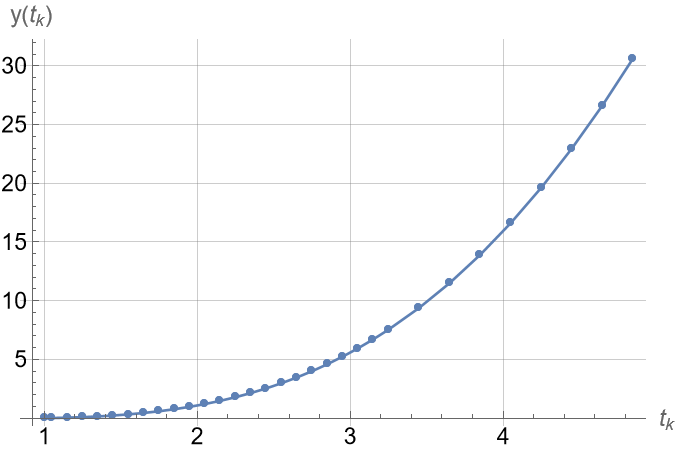
\includegraphics[width=0.7\textwidth]{auto_yk}
		\caption{Сеточное решение $y(t_k)$}
		\label{auto_yk}
	\end{figure}
	
	\begin{figure}[!h]
		\centering
		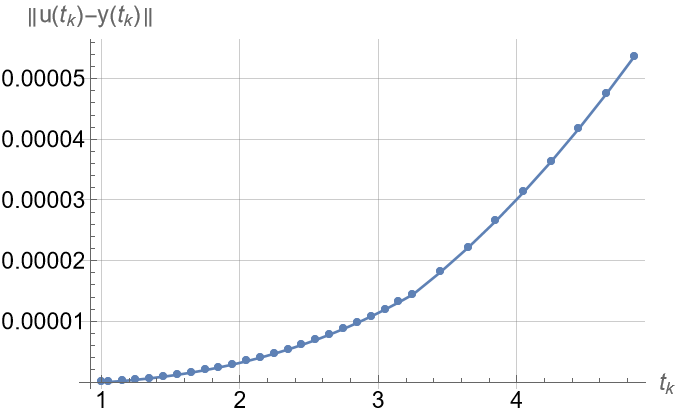
\includegraphics[width=0.7\textwidth]{auto_norm}
		\caption{Поточечная норма абсолютного отклонения $\|u(t_k) - y(t_k)\|$}
		\label{auto_norm}
	\end{figure}
	
	\begin{figure}[!h]
		\centering
		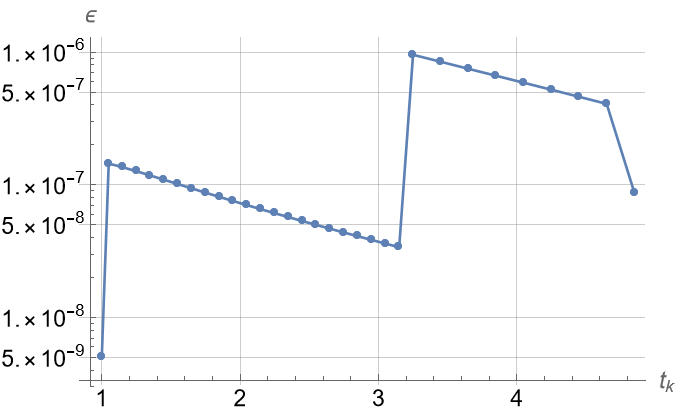
\includegraphics[width=0.7\textwidth]{auto_eps}
		\caption{Поточечная оценка локальной ошибки $\varepsilon$, полученной по правилу Рунге}
		\label{auto_eps}
	\end{figure}
	
	\begin{figure}[!h]
		\centering
		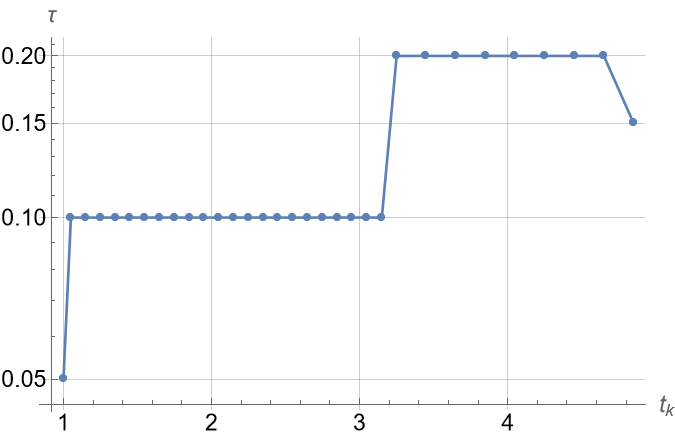
\includegraphics[width=0.7\textwidth]{auto_tau}
		\caption{Величина шага интегрирования $\tau$ в узлах $t_k$}
		\label{auto_tau}
	\end{figure}
	
	\subsection{Задача о маятнике}
	
	Уравнение математического маятника записывается в форме
	\[
	m \ddot{x} + kx = 0.
	\]
	
	Его можно привести к системе
	\[
	\begin{cases}
		u_1' = u_2, \\
		u_2' = - \omega^2 u_1,
	\end{cases}
	\]
	где $\omega^2 = \frac{k}{m}$. Данную систему можно записать в матричном виде:
	\[
	\begin{pmatrix} u_1' \\ u_2' \end{pmatrix} =
	G \begin{pmatrix} u_1 \\ u_2 \end{pmatrix}, \textrm{ где }
	G = \begin{pmatrix} 0 & 1 \\ -\omega^2 & 0 \end{pmatrix}.
	\]
	
	Исходное уравнение имеет вид $x(t) = r \cos(\omega t + \alpha)$, где $r$ и $\alpha$ --- амплитуда и начальная фаза колебаний соответственно. Т.е. в плоскости $(x, \dot{x})$ решение представляет собой эллипс.
	
	Воспользуемся численными методами для решения системы. Возьмем $\omega^2 = \frac{20}3$, $u_1(0) = u_2(0) = 1$. Явный метод Эйлера дает <<неустойчивый фокус>> (рис.~\ref{euler_expl_pend}). Черной точкой отмечено состояние системы в начальный момент времени.
	
	\begin{figure}[!h]
		\centering
		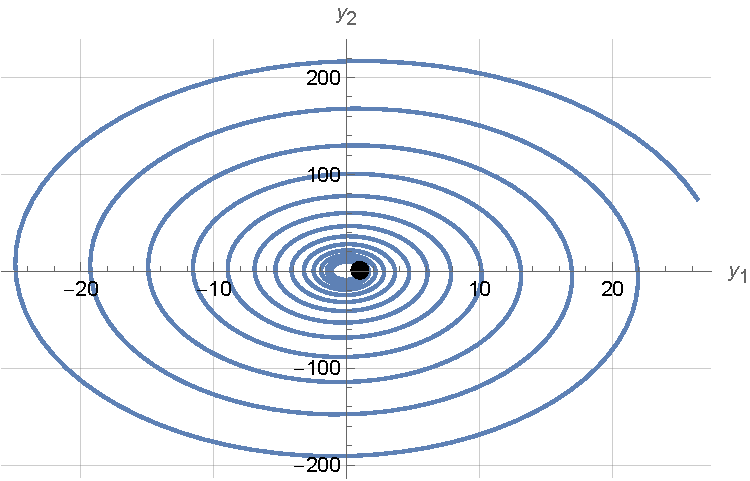
\includegraphics[width=0.7\textwidth]{euler_expl_pend}
		\caption{Решение уравнения математического маятника явным методом Эйлера}
		\label{euler_expl_pend}
	\end{figure}
	
	Явный метод Эйлера записывается в следующем виде:
	\begin{equation*}
		\frac{y_{n+1}-y_n}\tau = f(t_n, y_n) \textrm{ или } y_{n+1} = y_n + \tau f(t_n, y_n).
	\end{equation*}
	Применительно к текущей системе:
	\begin{equation*}
		\vec{y}_{n+1} = (E + \tau G) \vec{y}_n,
	\end{equation*}
	что также можно записать как
	\begin{equation*}
		\vec{y}_n = (E + \tau G)^n \vec{y}_0,
	\end{equation*}
	где $\vec{y}_0$ --- начальные условия.
	
	Матрица $G$ имеет два собственных значения $\lambda^{\pm} = \pm i \omega$, которым соответствуют два линейно независимых собственных вектора $\vec{v}^{\,+}$ и $\vec{v}^{\,-}$. Можно записать разложения вектора $\vec{y}_0$ по этому базису: $\vec{y}_0 = \alpha^+ \vec{v}^{\,+} + \alpha^- \vec{v}^{\,-}$. При условии, что $G \vec{v}^{\,+} = \lambda^+ \vec{v}^{\,+}$ и $G \vec{v}^{\,-} = \lambda^- \vec{v}^{\,+}$, выражение выше записывается так:
	\[
	\vec{y}_n = (1+\tau\lambda^+)^n \alpha^+ \vec{v}^{\,+} + (1+\tau\lambda^-)^n \alpha^- \vec{v}^{\,-}.
	\]
	
	Т.к. $|1+\tau \lambda^\pm| = \sqrt{1+ \omega^2 \tau^2} > 1$, то при $n \rightarrow \infty$ норма вектора $\vec{y}_n$ стремится к бесконечности. Вследствие этого наблюдается <<неустойчивым фокус>>.
	
	В случае неявного метода Эйлера получается график, представленный на рис.~\ref{euler_impl_pend}.
	
	\begin{figure}[!h]
		\centering
		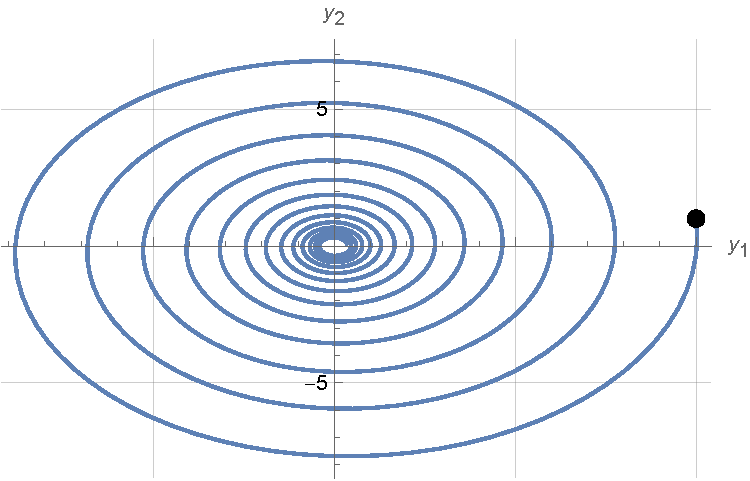
\includegraphics[width=0.7\textwidth]{euler_impl_pend}
		\caption{Решение уравнения математического маятника неявным методом Эйлера}
		\label{euler_impl_pend}
	\end{figure}
	
	В этом случае для математического маятника получается следующая запись:
	\[
	(E-\tau G) \vec{y}_{n+1} = \vec{y}_n.
	\]
	
	Если $\vec{y}_n = \alpha_1 \vec{v}^{\,+} + \alpha_2 \vec{v}^{\,-}$, $\vec{y}_{n+1} = \beta_1 \vec{v}^{\,+} + \beta_2 \vec{v}^{\,-}$, то приравняв соответствующие коэффициенты при собственных векторах, получаем уравнения, через которые можно выразить $\beta_1$ и $\beta_2$:
	\begin{equation*}
		\begin{cases}
			\beta_1 - \tau \lambda^+ \beta_1 = \alpha_1,\\
			\beta_2 - \tau \lambda^- \beta_2 = \alpha_2.
		\end{cases} \Rightarrow
		\begin{cases}
			\beta_1 = \dfrac1{1 - \tau \lambda^+} \alpha_1,\\
			\beta_2 = \dfrac1{1 - \tau \lambda^-} \alpha_2.
		\end{cases}
	\end{equation*}
	
	Используя полученные результаты, можно выписать общую формулу для $\vec{y}_n$:
	\begin{equation*}
		\vec{y}_n = \left(\dfrac1{1 - \tau \lambda^+}\right)^n \alpha^+ \vec{v}^{\,+} + \left(\dfrac1{1 - \tau \lambda^-}\right)^n \alpha^- \vec{v}^{\,-}.
	\end{equation*}
	
	Т.к. $\left|\sfrac1{1 - \tau \lambda^\pm}\right| = \sfrac1{\sqrt{1+ \tau^2 \omega^2}} < 1$, то в расчетах амплитуда колебаний затухает, из-за чего получается <<устойчивый фокус>>.
	
	% TODO еще картинки с другими результатами
	Для метода Рунге --- Кутты 2 порядка с расчетными формулами
	\[
	k_1 = f(t_n, y_n), \quad k_2 = f(t_n +\frac\tau2, y_n + \frac\tau2 k_1), \quad y_{n+1} = y_n + \tau k_2
	\]
	график представлен на рис.~\ref{rk2_pend}. Для того, чтобы показать, что график является <<неустойчивым фокусом>>, пришлось увеличить интервал интегрирования в 10 раз.
	
	\begin{figure}[!h]
		\centering
		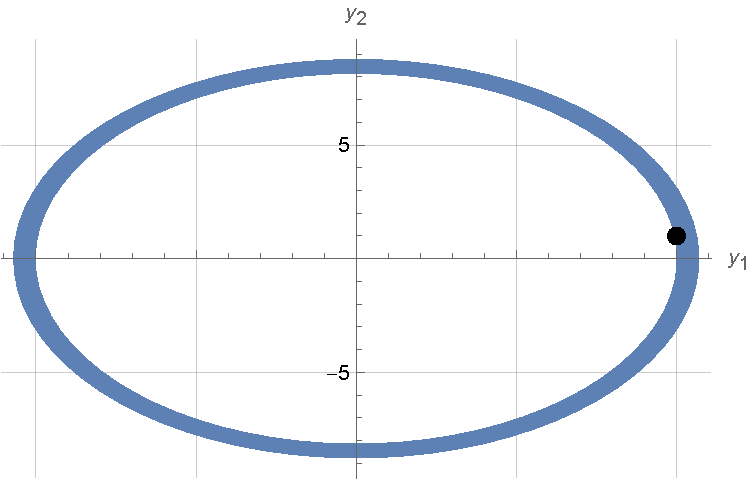
\includegraphics[width=0.7\textwidth]{rk2_pend}
		\caption{Решение уравнения маятника методом Рунге --- Кутты 2 порядка}
		\label{rk2_pend}
	\end{figure}
	
	Для математического маятника получаем, что
	\begin{equation*}
		\vec{k}_1 = G \vec{y}_n, \quad  \vec{k}_2 = G(\vec{y}_n + \frac\tau2 G \vec{y_n}) = (G + \frac\tau2 G^2)\vec{y_n}, \quad \vec{y}_{n+1} = \left(E + \tau G + \frac{\tau^2}2 G^2\right) \vec{y}_n.
	\end{equation*}
	
	Выражая через $\vec{y}_0$, приходим к следующему выражению:
	\begin{equation*}
		\vec{y}_n = \left(E + \tau G + \frac{\tau^2}2 G^2\right)^n \vec{y}_0.
	\end{equation*}
	
	Перепишем полученное равенство, используя разложение вектора $\vec{y}_0$:
	\begin{equation*}
		\vec{y}_n = \left(1 + \tau \lambda^+ + \frac{\tau^2}2 (\lambda^+)^2\right)^n \alpha^+ \vec{v}^{\,+} + \left(1 + \tau \lambda^- + \frac{\tau^2}2 (\lambda^-)^2\right)^n \alpha^- \vec{v}^{\,-}.
	\end{equation*}
	
	Аналогично найдем модули коэффициентов, находящихся под степенью:
	\begin{gather*}
		\left|1 + \tau \lambda^\pm + \frac{\tau^2}2 (\lambda^\pm)^2\right| = \sqrt{\left(1 - \frac{\tau^2 \omega^2}2\right)^2 + \tau^2 \omega^2} =\\= \sqrt{1 - 2\frac{\tau^2 \omega^2}2 + \frac{\tau^4 \omega^4}4 + \tau^2 \omega^2} 
		= \sqrt{1 + \frac{\tau^4 \omega^4}4} > 1.
	\end{gather*}
	
	Из-за того, что получившиеся коэффициенты больше 1, получается <<неустойчивый фокус>>, но в отличие от явного метода Эйлера скорость <<расхождения>> сильно меньше из-за большей степени у $\tau$, что и подтверждается экспериментально.
	
	Теперь исследуем симметричную схему:
	\begin{equation*}
		\frac{y_{n+1} - y_n}\tau = \frac{f(t_n, y_n) + f(t_n + \tau, y_{n+1})}2.
	\end{equation*}
	
	Фазовый портрет для маятника представлен на рис.~\ref{symml_pend}. Даже для увеличенного интервала интегрирования (в 10 раз по сравнению с метод Рунге --- Кутты) график всё равно представляет собой замкнутую траекторию, т.е. <<центр>>, который получается при аналитическом решении.
	
	\begin{figure}[!h]
		\centering
		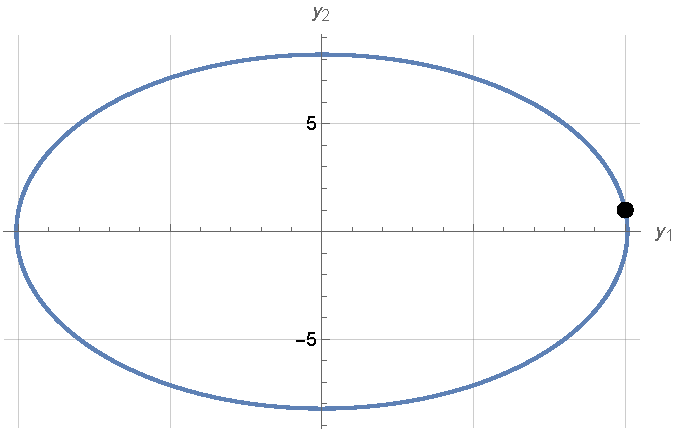
\includegraphics[width=0.7\textwidth]{symm_pend}
		\caption{Решение уравнения математического маятника симметричной схемой}
		\label{symml_pend}
	\end{figure}
	
	В случае маятника после группировки симметричная схема приобретает следующий вид:
	\begin{equation*}
		\left(E-\frac\tau2 G\right)\vec{y}_{n+1} = \left(E+\frac\tau2 G\right)\vec{y}_n.
	\end{equation*}
	
	Если $\vec{y}_n = \alpha_1 \vec{v}^{\,+} + \alpha_2 \vec{v}^{\,-}$, $\vec{y}_{n+1} = \beta_1 \vec{v}^{\,+} + \beta_2 \vec{v}^{\,-}$, то при подстановке в выражение приходим к системе:
	\begin{equation*}
		\begin{cases}
			\beta_1 - \frac\tau2 \beta_1 \lambda^+ = \alpha_1 + \frac\tau2 \alpha_1 \lambda^+, \\
			\beta_2 - \frac\tau2 \beta_2 \lambda^- = \alpha_2 + \frac\tau2 \alpha_2 \lambda^-.
		\end{cases} \Rightarrow
		\begin{cases}
			\beta_1 = \dfrac{2+\tau\lambda^+}{2-\tau\lambda^+}\alpha_1, \\[6pt]
			\beta_2 = \dfrac{2+\tau\lambda^-}{2-\tau\lambda^-}\alpha_2.
		\end{cases}
	\end{equation*}
	
	Таким образом,
	\begin{equation*}
		\vec{y}_n = \left(\frac{2+\tau\lambda^+}{2-\tau\lambda^+}\right)^n \alpha^+ \vec{v}^{\,+} + \left(\frac{2+\tau\lambda^-}{2-\tau\lambda^-}\right)^n \alpha^- \vec{v}^{\,-}.
	\end{equation*}
	
	При этом $\left|\dfrac{2+\tau\lambda^\pm}{2-\tau\lambda^\pm}\right| = 1$, следовательно, получаем устойчивое положение -- <<центр>>.
	
	\begin{table}[H]
		\caption{Шаг, обеспечивающий необходимую точность решения}
		\begin{center}
			\begin{tabular}{|c|c|c|c|}
				\hline
				\makecell{Метод}&$\varepsilon = 10^{-2}$&$\varepsilon = 10^{-4}$&$\varepsilon = 10^{-7}$\\
				\hline
				Эйлера (явный)& 3.71039e-06 & ---* & ---* \\
				\hline
				Эйлера (неявный)& 3.71039e-06 & ---* & ---* \\
				\hline
				Симметрическая схема& 0.00164759 & 0.000164628 & 5.20796e-06 \\
				\hline
				Рунге --- Кутта (2)& 0.00116539 & 0.000116467 & 3.68059e-06 \\
				\hline
				Рунге --- Кутта (4)& 0.0254059 & 0.00802755 & 0.00142097 \\
				\hline
				Адамса --- Башфорта& 0.00999832 & 0.00314903 & 0.000558615 \\
				\hline
				<<Прогноз-коррекция>>& 0.0182991 & 0.00599289 & 0.00106716 \\
				\hline
			\end{tabular}
		\end{center}
	\end{table}
	* Провести вычисления до достижения заданной точности не позволяют большой объем необходимой оперативной памяти и долгое время выполнения программы.
	
	
	\subsection{Исследование фазовой плоскости}
	
	Вариант 1, уравнение Ван-дер-Поля:
	\begin{equation*}
		\begin{cases}
			y''-2\delta y'(1.0-\alpha y^2)+\omega^2 y = 0,\\
			\delta = 0.3, \quad \omega = 1.0, \quad \alpha = 1.0, \\
			t = 0\dots200, \\
			y(0)=0.1, \quad y'(0)=0.1.
		\end{cases}
	\end{equation*}
	
	Приведем дифференциальное уравнение к системе заменой $y_1 = y$, $y_2 = y' = y_1'$. Тогда
	\begin{equation*}
		\begin{cases}
			y_1' = y_2, \\
			y_2' = 2\delta y_2(1.0-\alpha y_1^2) - \omega^2 y_1, \\
			\delta = 0.3, \quad \omega = 1.0, \quad \alpha = 1.0, \\
			t = 0\dots200, \\
			y_1(0)=0.1, \quad y_2(0)=0.1.
		\end{cases}
	\end{equation*}
	
	Найдем особые точки системы, приравняв правые части к нулю:
	\begin{equation*}
		\begin{cases}
			y_2 = 0, \\
			2\delta y_2(1.0-\alpha y_1^2) - \omega^2 y_1 = 0.
		\end{cases} \Rightarrow \quad
		\begin{cases}
			y_2 = 0, \\
			y_1 = 0.
		\end{cases}
	\end{equation*}
	Т.е. у системы одна особая точка, имеющая координаты $(0, 0)$.
	
	На рис.~\ref{part4_rk4}-\ref{part4_symm} представлены результаты численного решения системы тремя различными методами с двумя начальными условиями: $y_1(0)=0.1, y_2(0)=0.1$ и $y_1(0)= -0.1, y_2(0)=-0.1$. Все методы показали, что точка $(0, 0)$ является неустойчивой. Также по графикам видно, что у системы имеется также устойчивый аттрактор, называемый аттрактором Ван-дер-Поля (зеленые и красные кривые на графиках показывают сходимость к нему снаружи).
	
	\begin{figure}[!h]
		\centering
		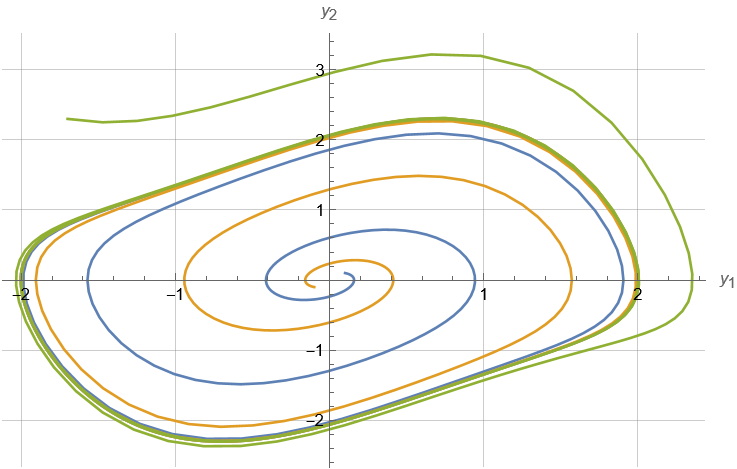
\includegraphics[width=0.6\textwidth]{part4_rk4}
		\caption{Решение системы методом Рунге --- Кутты 4 порядка}
		\label{part4_rk4}
	\end{figure}
	
	\begin{figure}[!h]
		\centering
		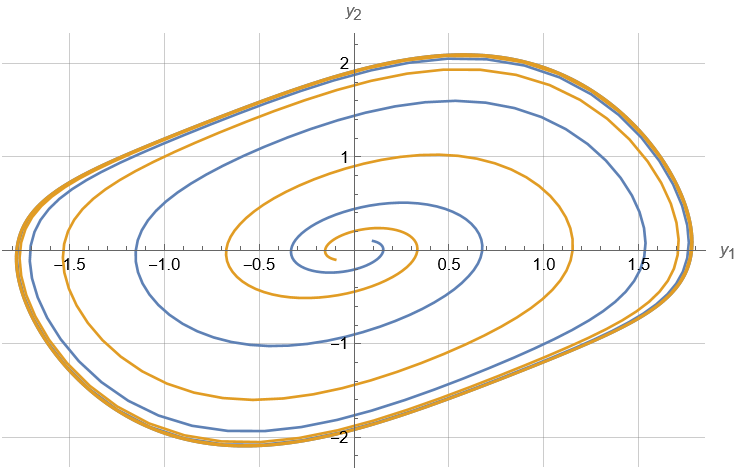
\includegraphics[width=0.6\textwidth]{part4_euler_impl}
		\caption{Решение системы неявным методом Эйлера}
		\label{part4_euler_impl}
	\end{figure}
	
	\begin{figure}[!h]
		\centering
		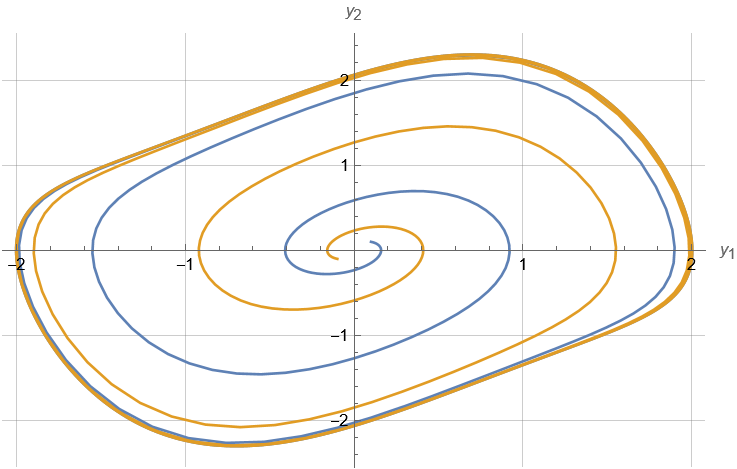
\includegraphics[width=0.6\textwidth]{part4_symm}
		\caption{Решение системы симметричной схемой}
		\label{part4_symm}
	\end{figure}
	
	Проверим это аналитически. Линеаризуем систему ДУ:
	\begin{equation*}
		\begin{cases}
			y_1' = y_2, \\
			y_2' = 2\delta y_2 - \omega^2 y_1, \\
			\delta = 0.3, \quad \omega = 1.0.
		\end{cases}
	\end{equation*}
	
	Собственные значения матрицы соответствующей системы:
	\begin{eqnarray*}
		& \begin{vmatrix}
			-\lambda  & 1                 \\
			-\omega^2 & 2\delta - \lambda
		\end{vmatrix} = \lambda^2 - 2 \delta\lambda + \omega^2 = 0, \\
		& D/4 = \delta^2 - \omega^2 < 0 \quad (\delta = 0.3, \omega = 1.0), \\
		& \lambda_{1,2} = \delta \pm i \sqrt{-D/4} \quad \Rightarrow \quad \mathrm{Re}\,\lambda_{1,2} > 0.
	\end{eqnarray*}
	
	Следовательно, по теореме Ляпунова об устойчивости по I приближению особая точка исходной системы является неустойчивой.
	
	% TODO физическая интерпретация
	% TODO выбор шага в многошаговых методах
	% TODO другие способы вывода условий порядка
	
	%\newpage
	\clearpage
	\begin{thebibliography}{1}
		\bibitem{galanin} \textit{Галанин М.П., Савенков Е.Б.} Методы численного анализа математических\\ моделей. М.: Изд-во МГТУ им. Н.Э. Баумана, 2010. 592 с.
		\bibitem{lukin} \textit{Галанин М.П., Лукин В.В., Щерица О.В.} Методы вычислений. Задачи алгебры и анализа. М.: Изд-во МГТУ им. Н.Э. Баумана, 2022. 376 с.
		
		
	\end{thebibliography}
	
	
\end{document}
